%%%%%%%%%%%%%%%%%%%%%%%%%%%%%%%%%%%%%%%%%%%%%%%%%%%%%%%%%%%%%%%%%%%%%%%%%%%%%%%

\chapter{DADOS ANALISADOS}

Este capítulo aborda as características gerais da Região Amazônica. Apresenta-se a seguir a descrição e relevância do projeto LBA. Finalizando, é realizada a descrição dos dados coletados pela campanha WETAMC do projeto LBA, como também do sítio experimental, durante tal campanha.

\section{A Amazônia}
\label{sec:amazonia}

O bioma\footnote{Corresponde a certos padrões de clima, formações geológicas, relevo, solo, hidrografia, vegetação e biodiversidade, com características paisagísticas bem definidas.}Amazônia ocupa $50\%$ da superfície da América do Sul, toda a porção norte, distribuída por nove países. Essa região é limitada a oeste pela Cordilheira dos Andes (com elevações de até $6.000$ metros), ao norte pelo Planalto das Guianas (com picos montanhosos de até $3.000$ metros), ao sul pelo Planalto Central (com altitudes típicas de $1.200$ metros) e ao leste pelo Oceano Atlântico. Em território brasileiro está mais da metade dos $6,9$ milhões de quilômetros quadrados originalmente cobertos por floresta~\cite{fisch/98}. 

Segundo o IBGE, aproximadamente $60\%$ da Floresta Amazônica pertence ao território brasileiro, que compreende a Amazônia Legal\footnote{Em $1953$, a Constituição Federal criou o conceito político de ``Amazônia Legal'', que representa $61\%$ do território brasileiro. Além dos sete estados da região Norte, inclui o estado do Mato Grosso e cerca de $79\%$ do estado do Maranhão}. Os $40\%$ restantes estão distribuídos entre os países da Bolívia, Colômbia, Equador, Guiana, Guiana Francesa, Peru, Suriname e Venezuela. 

Parte da vegetação na Amazônia sofre grande influência do processo de subida e descida das águas, o chamado pulso hidrológico. As florestas inundáveis representam $5$ a $10\%$ da área da Amazônia. São definidas por estarem alagadas durante parte do tempo, diariamente, no caso dos manguezais, ou alguns meses por ano, no caso das várzeas e igapós, ou mesmo durante todo o ano, como nos pântanos. 

As florestas de terra firme representam mais de $80\%$ da área amazônica. Tais florestas estão livres de inundações, já que ocupam terras mais altas com altitudes médias de $200$ metros. Esse tipo de floresta apresenta árvores de grande porte, que variam de $30$ a $60$ metros em altura. O dossel retém cerca de $95\%$ dos raios solares, o que torna o interior da floresta úmido e escuro. 

A convecção na região amazônica é um importante mecanismo de aquecimento da atmosfera tropical e sua variação, em termos de intensidade e posição, possue um papel importante na determinação do tempo e do clima desta região~\cite{fisch/98}. O clima é, em geral, quente e úmido e o comportamento da temperatura do ar apresenta uma pequena variação ao longo do ano. A amplitude térmica sazonal é da ordem de $1$-$2\,^{\circ}$C, sendo que os valores médios situam-se entre $24\,^{\circ}$ e $28\,^{\circ}$C.

A precipitação é um dos elementos climáticos mais importantes a ser analisado na região tropical, pois induz as características e comportamento de variáveis tais como temperatura, umidade relativa, vento etc. A região amazônica possui uma precipitação média de aproximadamente $2.300$ mm.ano$^{-1}$. O período de chuvas ou forte atividade convectiva na região amazônica é compreendido entre novembro a março, sendo que o período de seca (sem grande atividade convectiva) ocorre entre os meses de maio e setembro. Os meses de abril e outubro são meses de transição entre um regime e outro~\cite{fisch/98}.

O conhecimento das diversas componentes envolvidas na interação entre a biosfera e a atmosfera é fundamental para a previsão da evolução do clima, da sustentabilidade do ecossistema como um todo, assim como para a tomada de decisão sobre as políticas públicas mais adequadas para a minimização de impactos danosos irreversíveis~\cite{silvadias/05}. 

 
\section{O projeto LBA}

Nas últimas décadas, vários experimentos micrometeorológicos têm sido realizados na região amazônica, com o objetivo de aumentar os conhecimentos relativos à interação entre a floresta tropical e a atmosfera. Dentre os experimentos realizados destaca-se a campanha micrometeorológica intensiva do Projeto LBA (Experimento de Grande Escala de Interação Biosfera-Atmosfera na Amazônia). 

O projeto LBA é um grande programa de pesquisas liderado pelo Brasil e com cooperação científica internacional, composto por mais de $130$ projetos de pesquisas (já executados ou em fase de execução), financiados por várias agências nacionais (como o MCT, o CNPQ, a FAPESP, a FINEP/PPG7, etc) e internacionais (com destaques para a NASA e a National Science Foundation, dos EUA, a Comissão Européia, o IAI - Instituto Interamericano de Pesquisas de Mudanças Globais, etc)~\cite{nobre/2005}. 

As duas questões centrais do LBA são: (i) como funciona a Amazônia, na forma de um sistema regional, com respeito aos ciclos da água, energia, carbono, gases do efeito estufa e nutrientes?; e (ii) como as mudanças de uso da terra e do clima podem afetar o funcionamento físico, químico e biológico dos ecossistemas amazônicos? Estas questões levam em conta que as mudanças climáticas e ambientais têm efeito sobre o uso sustentável dos recursos naturais e, de uma forma geral, sobre as populações. Deste modo, o LBA visa auxiliar na definição de critérios de uso sustentável da floresta e do solo da Amazônia~\cite{nobre/2005}. 

A Figura~\ref{mapalocal} apresenta um mapa esquemático com as áreas de pesquisa de campo do LBA. As áreas principais fazem parte de duas transeções ecofisiológicas e de usos da terra. As áreas secundárias de pesquisa serão estabelecidas em toda a Amazônia.

\begin{figure}[ht]
	\caption{Mapa esquemático com a localização das áreas de pesquisa de campo do projeto LBA.}
	\vspace{6mm}	% acrescentar o espaçamento vertical apropriado entre o título e a borda superior da figura
	\begin{center}
		\resizebox{10.5cm}{!}{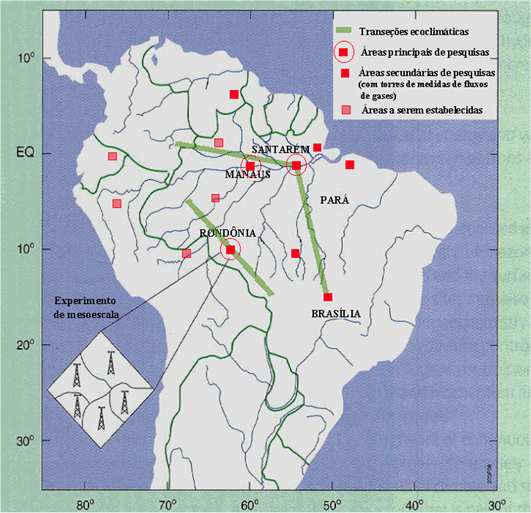
\includegraphics{Figuras/mapalbacorr.png}}		
	\end{center}
	\vspace{4mm}	% acrescentar o espaçamento vertical apropriado entre a borda inferior da figura e a legenda ou a fonte quando não há legenda (o valor pode ser negativo para subir)
	\legenda{Longitude em grau em abscisse e latitude em grau em ordenada.}	% legenda - para deixar sem legenda usar comando \legenda{} (nunca deve-se comentar o comando \legenda)
	\label{mapalocal}
	\FONTE{\citeonline{lba/06}.}	% fonte consultada (elemento obrigatório, mesmo que seja produção do próprio autor)
\end{figure}

\section{Sítio experimental e dados}
 
Os dados utilizados neste trabalho foram obtidos através de uma campanha micrometeorológica intensiva, a saber, WETAMC (Campanha de Mesoescala Atmosférica na Estação Úmida) que é parte do projeto LBA. Esta campanha foi realizada entre os meses de janeiro e março de 1999, na Reserva Biológica do Jaru ($10\,^{\circ}$46'S, $61\,^{\circ}$56'W), um sítio de floresta densa de aproximadamente $270$ mil hectares, pertencente ao Instituto Brasileiro do Meio Ambiente e dos Recursos Naturais Renováveis - IBAMA. Tal reserva está situada aproximadamente à $80$ Km ao norte de Ji-Paraná e a $120$ m acima do nível do mar, no estado de Rondônia, Brasil (ver Figura~\ref{rondonia}).  

\begin{figure}[ht]
	\caption{Mapa com a localização da campanha realizada pelo Projeto LBA.}
	\vspace{6mm}	% acrescentar o espaçamento vertical apropriado entre o título e a borda superior da figura
	\begin{center}
		\resizebox{11.5cm}{!}{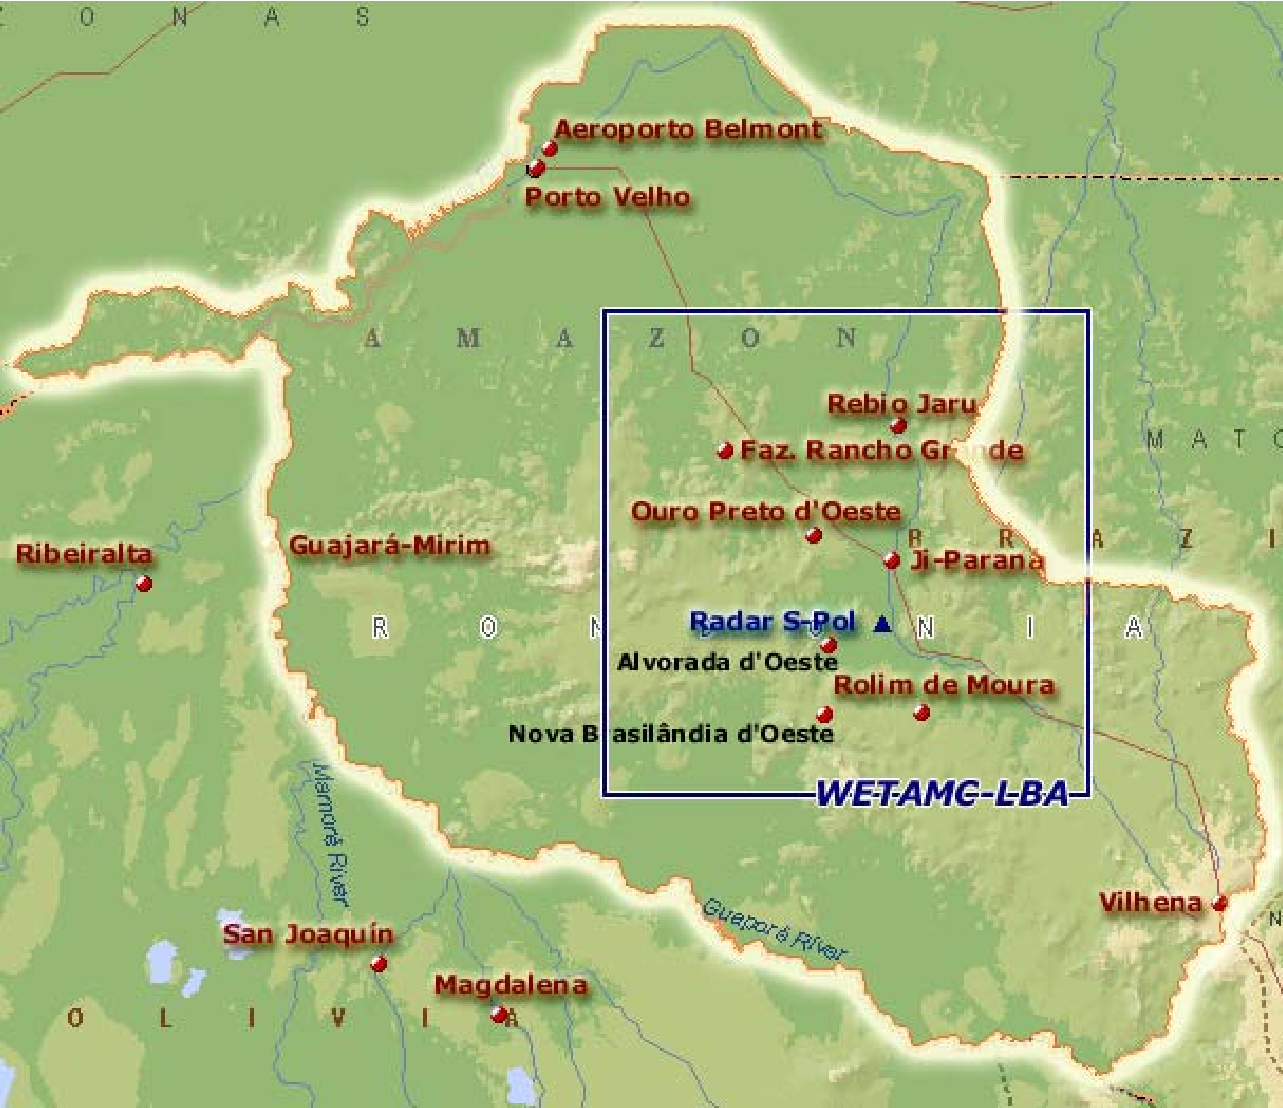
\includegraphics{Figuras/rondonia.pdf}}		
	\end{center}
		\vspace{2mm}	% acrescentar o espaçamento vertical apropriado entre a borda inferior da figura e a legenda ou a fonte quando não há legenda (o valor pode ser negativo para subir)
	\legenda{}	% legenda - para deixar sem legenda usar comando \legenda{} (nunca deve-se comentar o comando \legenda)
	\label{rondonia}
	\FONTE{\citeonline{iag/05}.}	% fonte consultada (elemento obrigatório, mesmo que seja produção do próprio autor)
\end{figure}

Uma estação meteorológica automática foi montada para medidas de resposta rápida de precipitação pluvial, temperatura do ar, umidade relativa do ar, velocidade e direção do vento, radiação solar incidente e de radiação de ondas longas emitida pela atmosfera e pela superfície, com médias coletadas em períodos de $30$ minutos, a uma freqüência de amostragem de $60$ Hz. Instrumentos como termômetros e anemômetros tridimensionais foram utilizados na área de floresta para medir tais variáveis meteorológicas e os fluxos de superfície (calor latente e calor sensível). 

As medidas foram feitas com o auxílio de uma torre micrometeorológica de alumínio de $66$ m de altura, simultaneamente em três diferentes alturas: Nível Superior ($66$ m - acima da copa); Nível Médio ($45$ m - no topo da copa); e Nível Inferior ($21$ m - abaixo da copa). 
A área onde tal torre foi construída está rodeada pela floresta amazônica de terra firme em um raio de pelo menos $800$ metros. As Figuras~\ref{torre} e \ref{figtorre} mostram, respectivamente, um desenho esquemático da torre e as vistas superior e inferior da mesma. Maiores informações do sítio experimental podem ser encontradas em \citeonline{culf/96}.

\begin{figure}[ht]
	\caption{Desenho esquemático da torre micrometeorológica do projeto LBA.}
	\vspace{6mm}	% acrescentar o espaçamento vertical apropriado entre o título e a borda superior da figura
	\begin{center}
		\resizebox{14cm}{!}{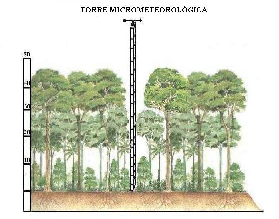
\includegraphics{Figuras/torredesenho.pdf}}		
	\end{center}
	\vspace{2mm}	% acrescentar o espaçamento vertical apropriado entre a borda inferior da figura e a legenda ou a fonte quando não há legenda (o valor pode ser negativo para subir)
	\legenda{}	% legenda - para deixar sem legenda usar comando \legenda{} (nunca deve-se comentar o comando \legenda)
	\label{torre}
	\FONTE{\citeonline{edtese/99}}.
\end{figure}

\begin{figure}[ht]
	\caption{Torre micrometeorológica de $66$ metros de altura construída na Reserva Biológica do Jaru (Rebio-Jaru), em Rondônia.}
	\vspace{6mm}	% acrescentar o espaçamento vertical apropriado entre o título e a borda superior da figura
	\begin{center}
		\resizebox{10.5cm}{!}{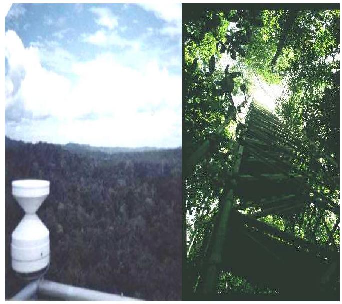
\includegraphics{Figuras/2torres.pdf}}		
	\end{center}
	\vspace{2mm}	% acrescentar o espaçamento vertical apropriado entre a borda inferior da figura e a legenda ou a fonte quando não há legenda (o valor pode ser negativo para subir)
	\legenda{À esquerda, vista superior; à direita, vista inferior.}	% legenda - para deixar sem legenda usar comando \legenda{} (nunca deve-se comentar o comando \legenda)
	\FONTE{\citeonline{iag/05}}.
	\label{figtorre}
\end{figure}

Dois períodos de medidas distintos foram selecionados: às 12 horas, quando a copa da floresta é aquecida pelo sol e o topo da mesma é mais quente que os arredores, e desta forma a região acima da copa é instável; e às 23 horas, quando as condições são opostas, e a região acima da copa é estável~\cite{Ramos/04}. Durante o experimento, o estado da atmosfera foi caracterizado pela existência de uma forte atividade convectiva no período diurno, com eventos de chuvas isoladas de dia e à noite.

É importante destacar que os dados obtidos através desta campanha foram submetidos a um rigoroso controle de qualidade conforme \citeonline{bolzan/00}. Desta forma, problemas freqüentemente encontrados em sinais experimentais, como por exemplo picos espúrios e vales, foram removidos dos mesmos.
